\documentclass[11pt,a4paper]{article}

\usepackage[margin=25mm]{geometry}
\usepackage[T1]{fontenc}
\usepackage{lmodern}
\usepackage{amsmath,amssymb}
\usepackage{booktabs,longtable,array}
\usepackage{hyperref}
\usepackage{enumitem}
\usepackage{tikz}
\usetikzlibrary{arrows.meta,positioning,shapes.geometric}

\hypersetup{colorlinks=true,urlcolor=blue,linkcolor=blue}
\setlength{\parindent}{0pt}
\setlength{\parskip}{0.65em}

\title{\textbf{From Candidate Hierarchy to Experimental Dependency Map}\\
\large Results from Five Preregistered Adversarial Tests of Maintenance, Heredity, Learning, Agency and Self-Modelling}
\author{Kenneth Craggs\\Independent Researcher, United Kingdom}
\date{16 October 2026\\Version 1.0.0\\DOI: \href{https://doi.org/10.5281/zenodo.23413881}{10.5281/zenodo.23413881}}

\begin{document}
\maketitle

\begin{abstract}
This paper synthesises the first completed preregistered experimental cycle of the Theory of Everything Research Programme. Five experimental blocks tested candidate relations involving dynamical persistence and maintenance, heredity and selection, retention--feedback--learning, structural generalisation and model-based agency, and reflective self-monitoring. Most mechanism-level hypotheses satisfied their preregistered criteria, but several serious bypass architectures also succeeded. Block I retained internal causal maintenance while reducing reciprocal-topology necessity. Block II retained heredity and selection within an artificial ecology while leaving robustness to alternative reproducing-unit definitions deferred. Block III retained separable causal roles for retention, feedback and learning while preserving information and control bypasses. Block IV retained a causal role for world-model content and counterfactual rollout in held-out structural novelty. Block V retained active self-monitoring, impairment-sensitive recovery, misinformation/correction rescue and self-specific capability tracking, restricted episode-specific correspondence, and reduced endogenous self-model necessity because externally supplied calibrated self-relevant information reproduced the registered downstream control function. The resulting architecture is not a validated ladder from physics to consciousness. It is a conditional dependency network containing scoped effective mechanisms, bypass routes and still-open transitions. In particular, the transitions from dissipative organisation to self-maintenance and from self-maintenance to reproduction remain unresolved, broad intelligence is not equated with one architecture, and phenomenal consciousness remains an independent open problem.
\end{abstract}

\noindent\textbf{Keywords:} Theory of Everything Research Programme; dependency architecture; adversarial experimentation; self-maintenance; heredity; natural selection; retention; feedback; learning; structural generalisation; world models; counterfactual rollout; self-monitoring; reflective control; bypass architectures; preregistration; open science.



\section{Introduction}

The Theory of Everything Research Programme was reformulated in Working Paper I as an adversarial search for the smallest empirically defensible explanatory architecture rather than an exercise in preserving a preferred unification. Working Paper II then rejected the assumption that one universal scalar of ``constraint'' could presently carry explanatory weight across all scales. Working Paper III converted the remaining dependency claims into five experimental blocks designed around matched controls, intervention, rescue, held-out novelty and serious bypass architectures.

The first complete experimental cycle is now available. Its scientific value does not lie in how many hypotheses received a favourable verdict. A retained result supports only the registered claim within the tested system. By contrast, a successful bypass can weaken a stronger necessity claim even when the original mechanism remains causally useful. Likewise, experimental success on capacities placed on either side of a proposed transition does not establish the transition itself.

Accordingly, this paper asks three questions. First, what did each block establish at its preregistered level? Second, which proposed dependencies survive once bypasses and scope limits are taken seriously? Third, what architecture should replace the provisional hierarchy after the evidence is returned to the dependency map of Working Paper I?

\section{Evidence standard and source record}

\paragraph{Publication status.}
This is the first public synthesis/results paper issued after completion of Experimental Blocks I--V. It reports and reconstructs the archived preregistered programme; it is not itself a new preregistered experiment. Cross-block judgements are therefore identified as synthesis-level inferences rather than retroactively preregistered hypotheses.


The foundational working papers are:
\begin{itemize}[leftmargin=*]
\item This synthesis/results paper: Zenodo \href{https://doi.org/10.5281/zenodo.23413881}{10.5281/zenodo.23413881}.
\item Working Paper I: \emph{From Physics to Consciousness? An Adversarial Search for a Minimal Explanatory Architecture}, DOI \href{https://doi.org/10.5281/zenodo.22857131}{10.5281/zenodo.22857131}.
\item Working Paper II: \emph{Constraint Across Scales: An Adversarial Test of Mathematical Unification}, DOI \href{https://doi.org/10.5281/zenodo.22857179}{10.5281/zenodo.22857179}.
\item Working Paper III: \emph{Testing a Candidate Dependency Architecture: An Adversarial Experimental Programme for Maintenance, Heredity, Learning, Agency and Self-Modelling}, DOI \href{https://doi.org/10.5281/zenodo.22857230}{10.5281/zenodo.22857230}.
\end{itemize}

Throughout the programme, \textbf{Retain} means that the relevant frozen criterion survived within its stated scope. \textbf{Restrict} narrows the domain of support. \textbf{Reduce} indicates that a stronger explanatory claim is defeated or subsumed by a simpler or alternative mechanism. \textbf{Deferred} or \textbf{Suspend} marks an unresolved test. None of these verdicts should be promoted automatically into a universal cross-scale law.

\section{Block I: persistence and causal maintenance}

Block I first separated persistent pattern formation from self-maintenance. The B1 Gray--Scott baseline was retained as a demonstration that sustained non-equilibrium driving can support persistent spatial organisation in the registered regime. No inference to life or autonomy followed.

B2 then tested a causal-maintenance network. H1.1--H1.4 were retained: active maintenance improved viability, internal maintenance survived withdrawal of external support, nominated reciprocal causal relations produced targeted failure propagation, and specific rescue restored the relevant function. H1.5 was initially deferred and later retained in a dedicated boundary/timescale follow-up. H1.6 was reduced because a budget-matched brute-force internal bypass met the registered non-inferiority conditions.

Quantitatively, passive-path viability was 20/20 under low, 14/20 under medium and 0/20 under high disturbance, whereas all four active architectures remained path-viable in 20/20 high-disturbance seeds. Following external-support withdrawal, external terminal viability was 4/20 while feed-forward, reciprocal and brute-force internal architectures were 20/20. The mean nominated C1-to-C2 ablation effect was 0.542929; specific rescue produced a mean C2 gain of 0.628158 compared with zero for irrelevant rescue.

The proper conclusion is therefore asymmetric. Internally generated maintenance is causally effective within the registered systems, but reciprocal topology is not necessary for the measured capacity. Moreover, B1 and B2 instantiate persistence and self-maintenance separately; they do not experimentally derive the latter from the former.

\section{Block II: heredity, reproduction and selection}

Block II retained H2.1, H2.2, H2.3, H2.4 and H2.6. H2.5 remained deferred because the ecology contained only one independently defensible reproducing unit.

Transmission fidelity in the E1 baseline was 0.9795, with conditional parent--offspring information 0.5679 nats compared with 0.0013 nats after shuffling. The E2 causal reproductive effect was 0.2797 expected offspring, with bootstrap 95\% interval 0.2384--0.3219. Favoured-variant final frequencies reached 0.9269 and 0.9288 in the registered selective ecologies. Following environmental reversal, the final adaptive-genotype frequency was 0.9231 for E2 versus 0.4950 for E1, and 20/20 E2 populations readapted within 35 generations.

These results support the restricted relation
\[
\text{reproduction + heredity + heritable variation + differential success}
\rightarrow
\text{selection-driven population change}.
\]
They do not establish the origin of reproduction from self-maintenance. The bridge from Block I to Block II therefore remains open even though the downstream evolutionary mechanism is experimentally instantiated.

\section{Block III: retention, feedback and learning}

All seven preregistered Block III hypotheses were retained. Policy-accessible retained state, within-episode feedback and between-episode learning produced distinct task-dependent causal effects.

Retention advantages on the history task were 0.4890, 0.4607 and 0.4249 at delays 4, 16 and 32, while the matched Markov effects were zero. Targeted retained-state interventions produced intact accuracy 0.9613, erase 0.4998, permute 0.4980 and opposite-state substitution 0.0377. Under unpredictable disturbance, closed-loop performance exceeded open-loop by 0.5340, yoked replay by 0.5748 and robust open-loop by 0.5340, while predictable disturbance produced no closed-loop advantage. Both held-out mapping families showed learning performance 1.0000 versus frozen-policy 0.0000, with post-freeze performance remaining 1.0000.

Bypasses constrain the interpretation. Direct present-state augmentation supplied the required history without online retention. Predictable disturbance allowed successful open-loop control. Explicit contextual mapping information produced correct changed-mapping behaviour without parameter learning.

Consequently, retention, feedback and learning are retained as separable effective mechanisms, not as a compulsory adaptive sequence.

\section{Block IV: structural generalisation and model-based agency}

Block IV retained H4.1--H4.7. Under held-out causal reversal, the model-based A3 architecture adapted in a median of one interaction compared with ten for A4PLUS, with 20/20 seeds favouring A3. In the consequence-depth tests, performance switched from failure to success exactly when the rollout horizon reached the decisive depth.

On held-out composition, A3 scored 1.00 compared with A2 0.05 and A4PLUS 0.15. On held-out problem-family novelty, A3 scored 1.00 compared with A2 0.00 and A4PLUS 0.10. Targeted world-model corruption reduced performance from 1.00 to 0.00 in both registered structural families, while irrelevant corruption left performance at 1.00. Correcting the corrupted relation restored performance to 1.00.

This conjunction is stronger than simple benchmark superiority because the internal model was manipulated causally. Even so, the result supports one model-based route to structural generalisation within the tested architecture family. It does not establish that all intelligent systems require explicit world models, nor that the registered tasks exhaust broad intelligence.

\section{Block V: causal self-related control}

Block V returned a deliberately mixed verdict: H5.1, H5.2, H5.3 and H5.5 were retained; H5.4 was restricted; H5.6 was reduced.

Active self-monitoring selectively improved behaviour over passive monitoring, assisted recovery after unannounced impairment, and showed the predicted causal failure-rescue sequence under direct misinformation and subsequent correction of the self-estimate. The endogenous self-monitor also tracked internal capability change better than world-only uncertainty.

Episode-specific monitor correspondence showed the predicted direction, but the mean effect did not satisfy both frozen H5.4 margins. More importantly, H5.6 reduced the endogenous-necessity claim because the H\_EXTERNAL bypass, supplied with calibrated self-relevant confidence from outside the endogenous monitor, remained within the preregistered utility margin while reproducing the downstream adaptive-control function.

The strongest defensible relation is therefore
\[
\text{accurate self-relevant information}
\rightarrow
\text{causal adaptive control},
\]
not
\[
\text{endogenous reflective self-model}
\Rightarrow
\text{necessary control architecture}.
\]

\section{Cross-block verdict matrix}

\small
\begin{longtable}{p{.12\linewidth}p{.36\linewidth}p{.43\linewidth}}
\toprule
Block & Registered outcome & Strongest surviving limitation\\
\midrule
\endhead
I & B1 Retain; H1.1--H1.4 Retain; H1.5 follow-up Retain; H1.6 Reduce & Persistence does not equal self-maintenance; reciprocal topology is not necessary; B1-to-B2 transition untested.\\
II & H2.1--H2.4 and H2.6 Retain; H2.5 Deferred & Reproduction-to-selection is supported once the population exists; self-maintenance-to-reproduction remains untested.\\
III & H3.1--H3.7 Retain & Information/control bypasses defeat universal necessity readings.\\
IV & H4.1--H4.7 Retain & Model-based causal route supported in registered structural-novelty tasks; universal intelligence/world-model necessity not established.\\
V & H5.1--H5.3, H5.5 Retain; H5.4 Restrict; H5.6 Reduce & External calibrated-confidence bypass defeats endogenous self-model necessity for the registered downstream function.\\
\bottomrule
\end{longtable}
\normalsize

\section{Evidence-driven reconstruction of the dependency map}

Working Paper I distinguished framework conditions, enabling conditions, effective mechanisms, transition problems and open problems. The five-block results now allow several entries to be sharpened without pretending that every transition has been solved.

\small
\begin{longtable}{p{.08\linewidth}p{.28\linewidth}p{.20\linewidth}p{.34\linewidth}}
\toprule
ID & Relation & Post-Block-V status & Evidence-driven judgement\\
\midrule
\endhead
FC1 & Physical states/histories $\rightarrow$ dynamical evolution & Unchanged framework & A modelling requirement, not a claim directly tested by Blocks I--V.\\
TP0 & Fundamental dynamics $\rightarrow$ stable matter/effective structure & Open unchanged & Outside the artificial five-block programme.\\
EC1 & Sustained driving $\rightarrow$ persistent dissipative organisation & Retain, scoped enabling condition & B1 provides an artificial example; no universal generator of complexity or life is established.\\
TP1 & Dissipative organisation $\rightarrow$ self-maintenance & Open, partially narrowed & Internal maintenance is causally demonstrable, but B1 was not transformed into B2; reciprocal-topology necessity was reduced.\\
EM1 & Historical distinction $\rightarrow$ consequential future influence & Retain, scoped & Block III retained causal retained-state use; direct current information can bypass retention.\\
TP2 & Self-maintenance $\rightarrow$ Darwinian population & Open & Block II begins with reproduction; the Block-I-to-Block-II bridge remains untested.\\
EM2 & Heritable variation + differential fitness $\rightarrow$ adaptive population change & Retain, scoped & Block II supports effective selection in the registered ecology.\\
EM3 & Perturbation-sensitive interaction $\rightarrow$ closed-loop regulation & Retain, scoped & Block III supports feedback when online correction is required; predictable conditions admit open-loop bypass.\\
EM4 & Experience $\rightarrow$ modified future behaviour & Retain, scoped & Block III supports learning; explicit context can bypass parameter updating.\\
TP3 & Adaptive regulation/learning $\rightarrow$ broad intelligent agency & Open, narrowed & Block IV supplies one causal route to structural generalisation, not a universal intelligence boundary.\\
TP4 & Intelligent agency $\rightarrow$ reflective self-modelled intelligence & Open, narrowed & Block V supports causal self-related control; endogenous self-model necessity is reduced and the Block-IV-to-Block-V dependency itself was not tested.\\
OP1 & Physical/biological organisation $\rightarrow$ phenomenal consciousness & Open unchanged & No Block I--V experiment measured phenomenality or validated a bridge to subjective experience.\\
\bottomrule
\end{longtable}
\normalsize

\section{The revised topology}

The most important programme-level result is the failure of a compulsory ladder. Figure~\ref{fig:map} represents the post-Block-V architecture schematically.

\begin{figure}[ht]
\centering
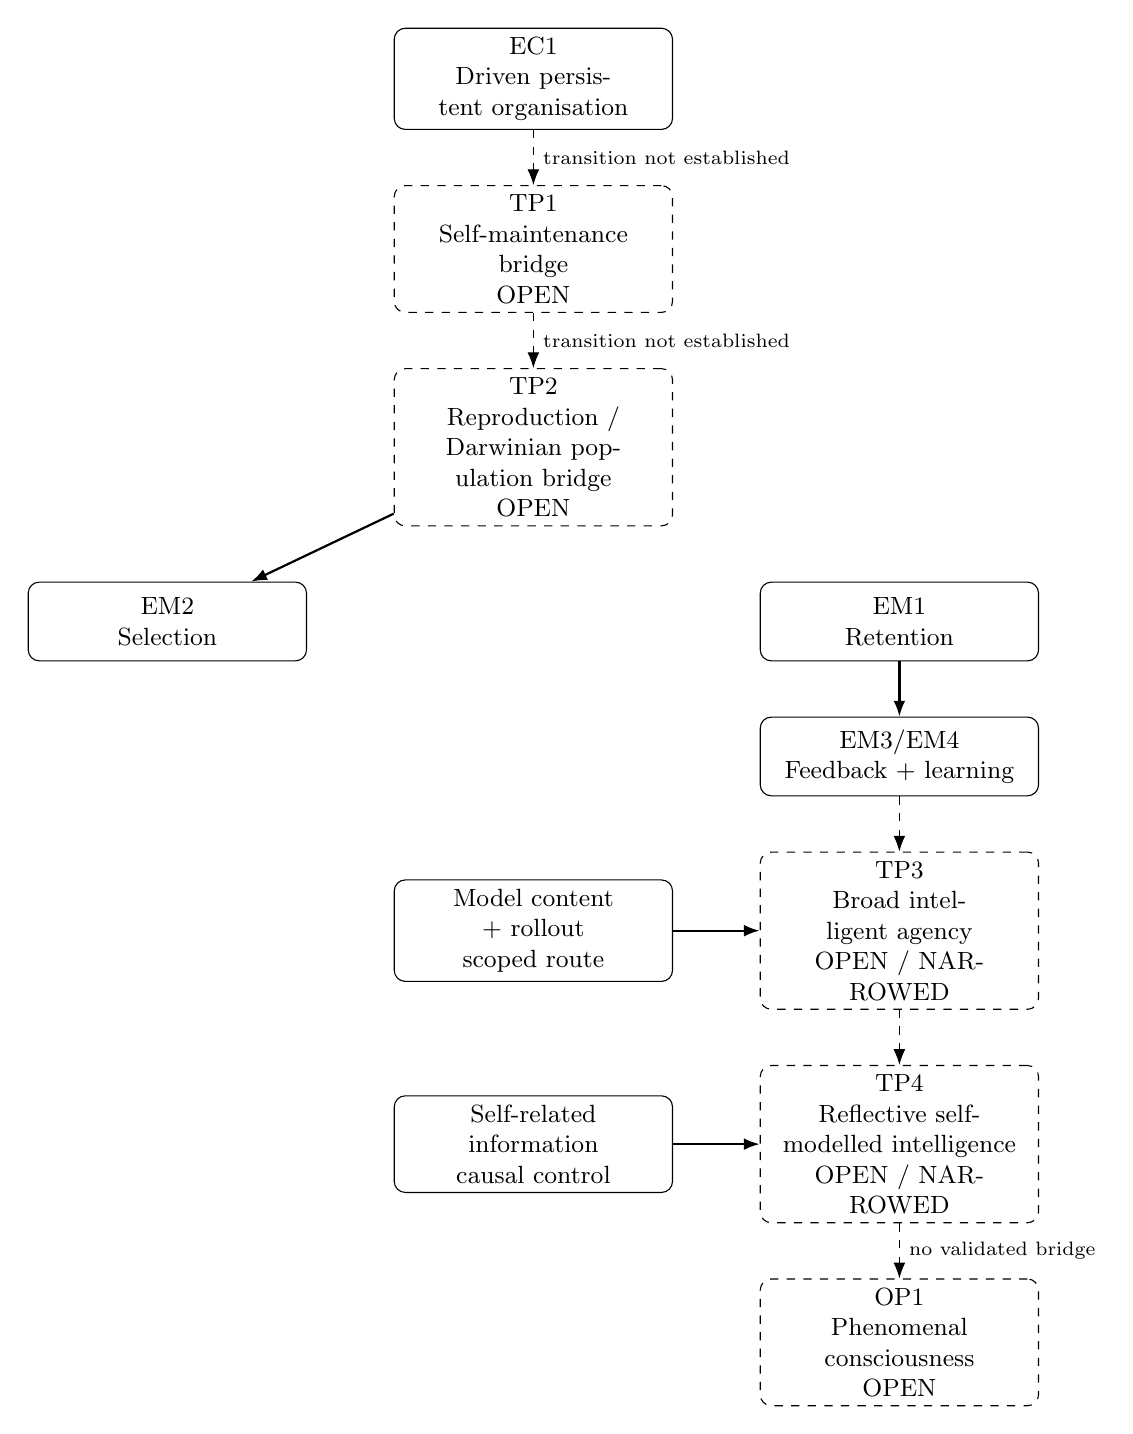
\begin{tikzpicture}[
node distance=7mm and 11mm,
box/.style={draw,rounded corners,align=center,text width=33mm,minimum height=10mm,font=\small},
open/.style={draw,dashed,rounded corners,align=center,text width=33mm,minimum height=10mm,font=\small},
arr/.style={-{Latex[length=2mm]},thick},
dasharr/.style={-{Latex[length=2mm]},dashed}
]
\node[box] (ec1) {EC1\\Driven persistent organisation};
\node[open,below=of ec1] (tp1) {TP1\\Self-maintenance bridge\\OPEN};
\node[open,below=of tp1] (tp2) {TP2\\Reproduction / Darwinian population bridge\\OPEN};
\node[box,below left=of tp2] (em2) {EM2\\Selection};
\node[box,below right=of tp2] (em1) {EM1\\Retention};
\node[box,below=of em1] (em34) {EM3/EM4\\Feedback + learning};
\node[open,below=of em34] (tp3) {TP3\\Broad intelligent agency\\OPEN / NARROWED};
\node[box,left=of tp3] (wm) {Model content\\+ rollout\\scoped route};
\node[open,below=of tp3] (tp4) {TP4\\Reflective self-modelled intelligence\\OPEN / NARROWED};
\node[box,left=of tp4] (selfinfo) {Self-related information\\causal control};
\node[open,below=of tp4] (op1) {OP1\\Phenomenal consciousness\\OPEN};

\draw[dasharr] (ec1) -- node[right,font=\scriptsize]{transition not established} (tp1);
\draw[dasharr] (tp1) -- node[right,font=\scriptsize]{transition not established} (tp2);
\draw[arr] (tp2) -- (em2);
\draw[arr] (em1) -- (em34);
\draw[dasharr] (em34) -- (tp3);
\draw[arr] (wm) -- (tp3);
\draw[dasharr] (tp3) -- (tp4);
\draw[arr] (selfinfo) -- (tp4);
\draw[dasharr] (tp4) -- node[right,font=\scriptsize]{no validated bridge} (op1);
\end{tikzpicture}
\caption{Post-Block-V dependency architecture. Solid arrows indicate scoped experimentally supported causal routes. Dashed arrows mark transitions that remain open or were not directly tested as cross-block dependencies.}
\label{fig:map}
\end{figure}

Several consequences follow. Selection can operate without explaining the origin of reproduction. Feedback and learning can contribute to adaptive control without constituting intelligence. Model-based rollout can contribute causally to structural novelty without becoming a universal law of intelligence. Self-related information can regulate behaviour without requiring endogenous generation of that information. Phenomenal consciousness remains outside the validated functional chain.

\section{Mechanism efficacy versus dependency necessity}

The experiments repeatedly distinguish two propositions:
\[
M \text{ causally helps produce } Y
\]
and
\[
Y \Rightarrow M.
\]
Blocks I, III and V provide particularly clear counterexamples to conflating them. Internal causal maintenance can help preserve viability while reciprocal topology is unnecessary. Retention, feedback and learning can each matter while task-relevant information or predictable dynamics allow bypasses. Endogenous self-monitoring can guide control while externally supplied calibrated self-relevant information reproduces the registered function.

This distinction should become part of the permanent ToE methodology. Effective mechanisms earn inclusion because they perform identifiable causal work. Necessity claims require separate adversarial tests and should be withdrawn or narrowed when a serious bypass succeeds.

\section{What remains unresolved}

The first cycle leaves several major questions open.

\paragraph{TP1.} The programme has not demonstrated how persistent dissipative organisation becomes causally integrated self-maintenance. Future work must attack this transition in chemical and biological systems rather than infer it from artificial maintenance alone.

\paragraph{TP2.} The origin of reproduction, lineage continuity and heritable population structure from self-maintaining organisation remains unresolved. Block II validates selection only after these prerequisites have been supplied.

\paragraph{TP3.} Structural generalisation is a useful discriminator of broader agency, and Block IV supplies one strong causal model-based route. A general theory of intelligence, however, would require broader architecture classes, domains and resource-matched alternatives.

\paragraph{TP4.} Causal self-related control is experimentally tractable, but Block V does not establish that endogenous reflective self-modelling is universally required. The external-confidence bypass makes that limitation explicit.

\paragraph{OP1.} No five-block result closes the consciousness problem. Self-monitoring, self-report, causal self-model use and structural generalisation remain functional capacities, not validated measures of phenomenality.

\section{Implications for Working Papers I--III}

Working Paper I should now be read with a sharper distinction between retained mechanisms and unresolved bridges. EM1--EM4 receive direct artificial-system support at restricted scopes. TP1--TP4 remain transition problems, although TP3 and TP4 are narrowed by successful artificial routes.

Working Paper II is strengthened methodologically rather than vindicated as a universal theory of constraint. The experiments repeatedly required different measures, baselines and causal interventions. Nothing in the five-block cycle supplies evidence for collapsing these quantities into one universal constraint scalar.

Working Paper III has now completed its principal empirical purpose. The block structure proved useful as an experimental organisation, but the resulting evidence does not reproduce the blocks as a compulsory hierarchy. That is a positive result: the protocol successfully allowed bypasses, restrictions and reductions to alter the architecture.

\section{Phenomenal consciousness remains Open Problem 1}

The functional-developmental sequence and the consciousness question should remain bifurcated. Block V shows that a system can use information about its own reliability causally. It does not show that such a system has subjective experience, and the successful external-confidence bypass further weakens any simple identification of endogenous self-monitoring with phenomenality.

A future OP1 programme should therefore begin from competing consciousness hypotheses and theory-specific discriminating predictions rather than add a sixth artificial ``consciousness block''. The evidential target is a validated bridge between physical or organisational properties and phenomenal state, not another behavioural capacity placed above self-modelling.

\section{Conclusion}

The first five-block confirmatory cycle transforms the ToE programme from a candidate hierarchy into an experimentally constrained dependency map. The strongest surviving claims are local and causal: internal maintenance can preserve operation; heredity and differential reproductive success can drive population change; retention, feedback and learning can make separable contributions; world-model content and rollout can causally support structural generalisation; and self-related information can regulate behaviour.

Equally important are the results that remove structure. Reciprocal maintenance topology is not necessary for the registered maintenance capacity. Several adaptive mechanisms admit informational or control bypasses. Endogenous self-modelling is not necessary for the registered downstream self-related control function. The transitions connecting major organisational levels remain less established than the mechanisms operating within those levels.

The resulting Theory of Everything architecture is therefore not a ladder culminating in consciousness. It is a conditional network of framework conditions, enabling conditions, effective mechanisms, bypass routes and unresolved transitions. Progress now consists in attacking the remaining bridges with the same discipline that allowed the original hierarchy to be weakened where the evidence required it.


\section{Open Science, Data and Code Availability}

The five-block experimental programme was conducted through public preregistration, frozen machine-readable manifests, held-out confirmatory seeds, versioned software releases, raw or per-seed confirmatory records, reproducible analyses and explicit decision records. The primary OSF and Zenodo records are listed below.

This synthesis paper introduces no new experimental dataset. Its evidential basis is the archived Block I--V record. The machine-readable five-block synthesis and post-Block-V dependency map accompanying this paper are derived summaries of those public records.

The publication DOI for this synthesis is \href{https://doi.org/10.5281/zenodo.23413881}{10.5281/zenodo.23413881}. The source \LaTeX, compiled PDF, machine-readable synthesis record and machine-readable dependency map are preserved with the publication package.


\section*{Primary research record}

\begin{itemize}[leftmargin=*]
\item Block I B1: OSF \href{https://doi.org/10.17605/OSF.IO/G3TE5}{G3TE5}; software \href{https://doi.org/10.5281/zenodo.23075692}{23075692}; dataset \href{https://doi.org/10.5281/zenodo.23075718}{23075718}.
\item Block I B2: OSF \href{https://doi.org/10.17605/OSF.IO/GQANP}{GQANP}; software \href{https://doi.org/10.5281/zenodo.23122125}{23122125}; dataset \href{https://doi.org/10.5281/zenodo.23122412}{23122412}.
\item Block I H1.5 follow-up: OSF \href{https://doi.org/10.17605/OSF.IO/JRCNB}{JRCNB}; software \href{https://doi.org/10.5281/zenodo.23137073}{23137073}; dataset \href{https://doi.org/10.5281/zenodo.23137082}{23137082}.
\item Block II: OSF \href{https://doi.org/10.17605/OSF.IO/EUF2J}{EUF2J}; software \href{https://doi.org/10.5281/zenodo.23236866}{23236866}; dataset \href{https://doi.org/10.5281/zenodo.23236897}{23236897}.
\item Block III: OSF \href{https://doi.org/10.17605/OSF.IO/8ZWM7}{8ZWM7}; software \href{https://doi.org/10.5281/zenodo.23244848}{23244848}; dataset \href{https://doi.org/10.5281/zenodo.23244857}{23244857}.
\item Block IV: OSF \href{https://doi.org/10.17605/OSF.IO/REHW5}{REHW5}; software \href{https://doi.org/10.5281/zenodo.23263492}{23263492}; dataset \href{https://doi.org/10.5281/zenodo.23263512}{23263512}.
\item Block V: OSF \href{https://doi.org/10.17605/OSF.IO/JZ4ED}{JZ4ED}; software \href{https://doi.org/10.5281/zenodo.23321474}{23321474}; dataset \href{https://doi.org/10.5281/zenodo.23321507}{23321507}.
\end{itemize}

\end{document}
